% !TEX root =  ../main_manuscript.tex 
\section{Personalized Schedule of Invasive Tests for Detecting Progression}
\label{sec:schedule}
We intend to develop a personalized schedule of invasive tests for a new patient $j$, not present in training dataset $\mathcal{A}_n$. Tests are conducted only until progression is detected (Figure~\ref{fig:delay_explanation}). Let $T^*_j$ be the true time of progression, and ${t < T^*_j}$ be the time of the last test on which progression was not detected for the $j$-th patient. Lastly, ${v \geq t}$ denotes the time of the current follow-up visit.

\subsection{Cumulative-risk of progression}
\label{subsec:cum_risk}
First we combine the history of observed longitudinal outcomes $\{\mathcal{Y}_{1j}(v), \ldots, \mathcal{Y}_{Kj}(v)\}$ until the current visit time $v$, and the previous negative test result ${T^*_j > t}$ to define the patient-specific cumulative-risk of progression at future time $u$ (Figure~\ref{fig:dynrisk_explanation}).
\begin{equation}
\label{eq:cumulative_risk}
\begin{split}
R_j(u \mid t, v) &= \mbox{Pr}\big\{T^*_j \leq u \mid T^*_j > t, \mathcal{Y}_{1j}(v), \ldots, \mathcal{Y}_{Kj}(v), \mathcal{A}_n\big\}\\
&=\int \int \mbox{Pr}(T^*_j \leq u \mid T^*_j > t, \boldsymbol{b}_{j}, \boldsymbol{\theta}) p\big\{\boldsymbol{b}_j \mid T^*_j > t, \mathcal{Y}_{1j}(v), \ldots, \mathcal{Y}_{Kj}(v), \boldsymbol{\theta} \big\}\\
&\quad \times p(\boldsymbol{\theta} \mid \mathcal{A}_n) \mathrm{d}\boldsymbol{b}_j \mathrm{d}\boldsymbol{\theta}, \quad u \geq t.
\end{split}
\end{equation}
The personalized cumulative-risk function $R_j(\cdot)$ depends on the observed longitudinal data $\{\mathcal{Y}_{1j}(v), \ldots, \mathcal{Y}_{Kj}(v)\}$, and the training dataset $\mathcal{A}_n$ via the posterior distribution of patient-specific random effects~$\boldsymbol{b}_j$, and posterior distribution of the vector of joint model parameters~$\boldsymbol{\theta}$, respectively. The risk also dynamically updates as more longitudinal data becomes available over follow-up (Panel~B~and~C, Figure~\ref{fig:dynrisk_explanation}).

\begin{figure}
\centerline{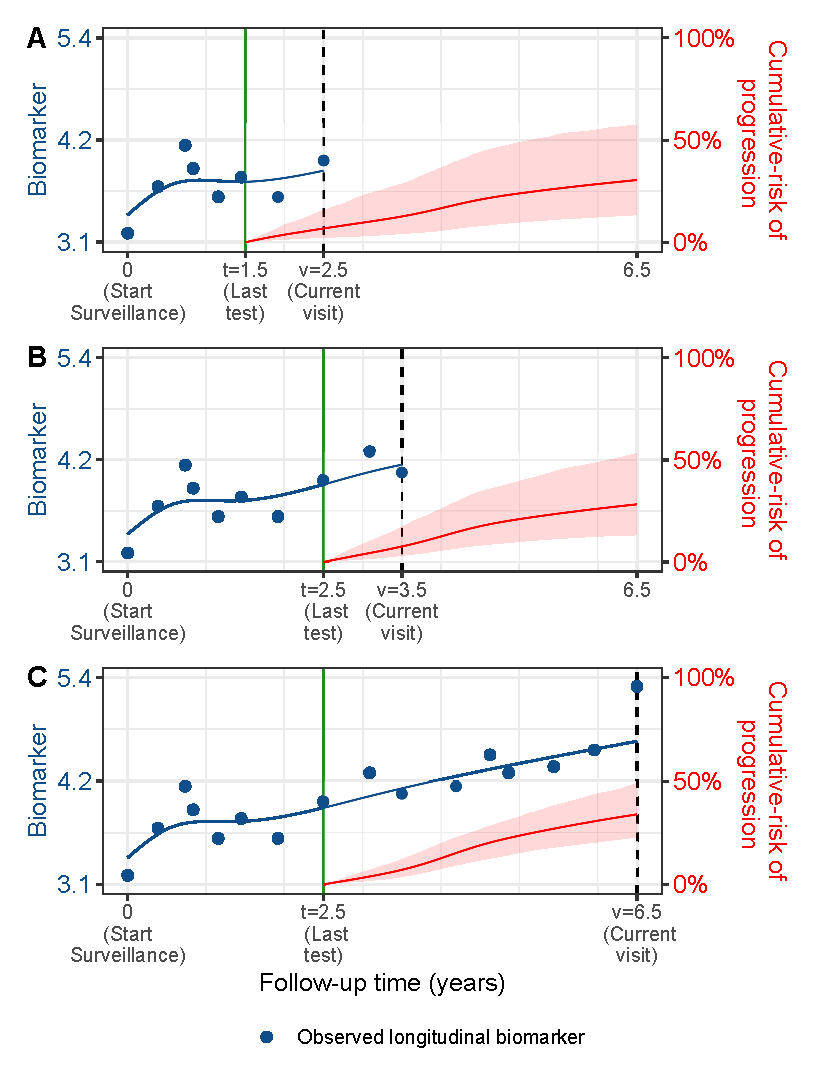
\includegraphics{images/dynrisk_plot_102.eps}}
\caption{\textbf{Cumulative-risk of progression changing dynamically over follow-up} as more patient data is gathered. A single longitudinal outcome, namely, a continuous biomarker of disease progression, is used for illustration. \textbf{Panels~A,~B~and~C:} are ordered by the time of the current visit (dashed vertical black line) of a new patient. At each of these visits, we combine the accumulated longitudinal measurements (shown in blue), and last time of negative invasive test (solid vertical green line) to obtain the updated cumulative-risk profile (shown in red) of the patient. All values are illustrative.} 
\label{fig:dynrisk_explanation}
\end{figure}

\subsection{Schedule of Invasive Tests}
\label{subsec:pers_schedule}
Our aim is to employ the cumulative-risk function in~(\ref{eq:cumulative_risk}) to develop a personalized schedule of invasive tests for the $j$-th patient. Typically invasive tests are planned on the same visit on which auxiliary data (e.g., biomarkers) is measured. Let $U={u_1, \ldots, u_L}$ represent a schedule of such visits (e.g., every six months in prostate cancer for PSA measurement), where $u_1=v$ is also the time of the current visit. In addition, $u_1 > t$, the time of the last test on which progression was not observed. We then propose scheduling future tests on all those visits in $U$ where the conditional cumulative-risk of progression is larger than a certain threshold $0 \leq \kappa \leq 1$ (e.g., $\kappa=10$\% risk). Each such future decision of a test at time $u_l \in U$ is given by:
\begin{equation*}
\label{eq:personalized_decision_grid}
\begin{split}
D_j(u_l \mid t_l, v, \kappa) &= I\big\{R_j(u_l \mid t_l, v) \geq \kappa \big\},\\
t_{l} &= \max \big\{t, u_m \mid D_j(u_m \mid t_m, v, \kappa)=1, m=1,\ldots,l-1 \big\}
\end{split}
\end{equation*}
where $D_j(u_l \mid t_l, v, \kappa)$ denotes the test decision at future visit time $u_l$, with 1 representing a test planned at $u_l$ and 0 otherwise, and $I(\cdot)$ is the corresponding indicator function. The conditional cumulative-risk of progression denoted by $R_j(u_l \mid t_l, v)$ is defined as in~(\ref{eq:cumulative_risk}). It is called `conditional' because test decision at each successive future visit time $u_l$ is made by accounting for the possibility that progression may not occur until the time of the last planned test $t_l$. That is, $T^*_j > t_l$. However, the contribution of the observed longitudinal data $\{\mathcal{Y}_{1j}(v), \ldots, \mathcal{Y}_{Kj}(v)\}$ does not change while making these consecutive decisions. The personalized schedule of tests $S_j^\kappa$ for a given risk threshold $\kappa$ is then defined as the subset of time points in $U$ on which tests are planned, until progression is observed or we reach a maximum horizon $h$.
\begin{equation*}
\label{eq:personalized_schedule_grid}
S_j^\kappa = \Big\{ u_l \in U \mid D_j(u_l \mid t_l, v, \kappa)=1, u_l < T^*_j, u_l<h \Big\}
\end{equation*}
Since the schedule is risk based, it also gets updated as more patient data becomes available over follow-up.

\begin{figure}
\centerline{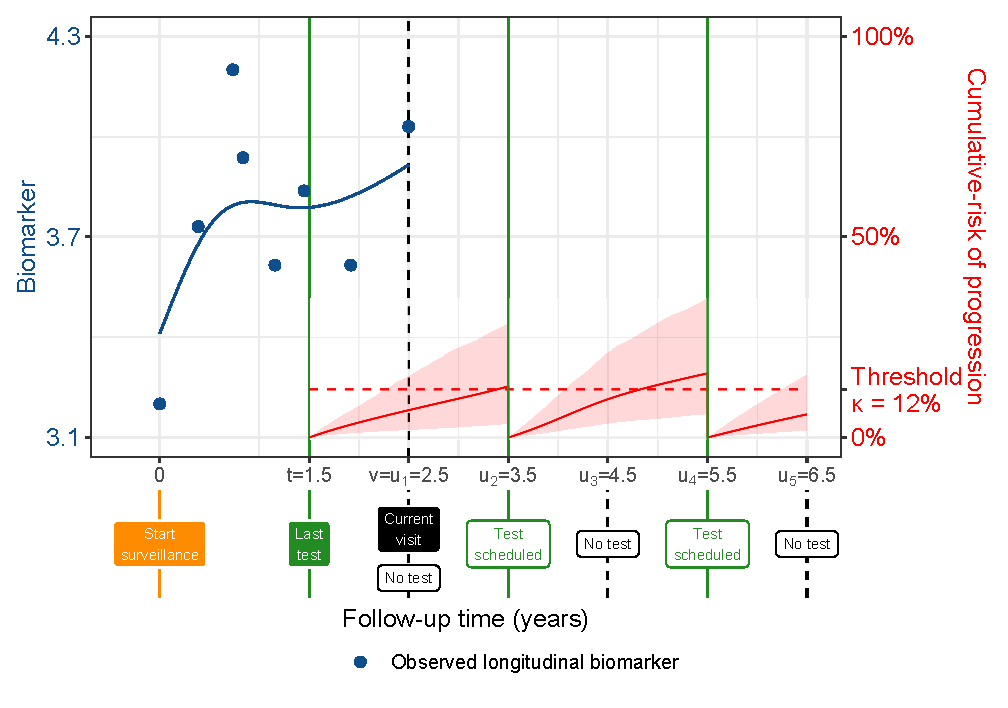
\includegraphics{images/schedule_explanation_102.eps}}
\caption{\textbf{Personalized Invasive Test Schedule Using Patient-specific Conditional Cumulative-risk of Progression}.  A single longitudinal outcome, namely, a continuous biomarker (observed: blue dots, fitted: blue line) of disease progression is used for illustration. The last test on which progression was not observed was conducted at $t=1.5$ years. The current visit time of the patient is $v=2.5$ years. Decisions for invasive test need to be made at a gap of every one year starting from the current visit until a horizon of 6.5 years. That is, $U=\{2.5, 3.5, 4.5, 5.5, 6.5\}$ years. Based on an example risk threshold of 12\% ($\kappa=0.12$) the future test decisions at time points in $U$ lead to a personalized schedule $S_j^\kappa = (3.8, 5.7)$ years. The conditional cumulative-risk profiles $R_j(u_l \mid t_l, v)$ employed in~(\ref{eq:personalized_decision_grid}) are shown with red line (confidence interval shaded). It is called `conditional' because, for example, the second test at future time 5.5 years, is scheduled after accounting for the possibility that progression (true time $T^*_j$) may not have occurred until the time of the previously scheduled test at time $3.5 < T^*_j$ years. All values are illustrative.} 
\label{fig:schedule_explanation}
\end{figure}

\subsection{Risk Threshold $\kappa$}
The risk threshold $\kappa$ controls the timing and the total number of invasive tests in the schedule $S_j^{\kappa}$. Through the timing of tests, $\kappa$ also indirectly affects the time delay (Figure~\ref{fig:delay_explanation}) that may occur in detecting progression if this schedule is followed. Hence, $\kappa$ should be chosen while balancing both the number of invasive tests (burden) and the time delay in detecting progression (less is beneficial).

Consider the bi-dimensional Euclidean space of the total number of invasive tests (x-axis) and the corresponding expected time delay in detecting progression (y-axis) for schedules associated with various $\kappa$ (Figure~\ref{fig:kappa_choice}). An ideal schedule of tests will have only one test planned exactly at the true time of progression $T^*_j$ of a patient. In other words, it will lead to a zero time delay. This schedule is shown at the point of optimality (1, 0) in Figure~\ref{fig:kappa_choice}. Subsequently, a threshold $\kappa_a$ can be chosen automatically by minimizing the Euclidean distance between the point $(1,~0)$ and the set of points representing various schedules corresponding to each $0 \leq \kappa \leq 1$. That is,
\begin{equation}
\label{eq:kappa_choice}
\kappa_a = \argmin_{\kappa} \sqrt{\big(\vert S_j^\kappa \vert - 1\big)^2 + \Big[E\{Q_j(S_j^{\kappa}, t)\} - 0\Big]^2} , \quad 0 \leq \kappa \leq 1,
\end{equation}
where, $E\{Q_j(S_j^{\kappa}, t)\}$ denotes the expected value of the time delay $Q_j(S_j^{\kappa}, t)$ in detecting progression if schedule $S_j^{\kappa}$ is followed. Additional consequences of following a particular schedule, such as (quality-adjusted) life-years saved, can also be accommodated in~(\ref{eq:kappa_choice}). This can be achieved by first setting a point of optimality in a higher dimensional Euclidean space of the aforementioned consequences, and then minimizing the Euclidean distance to the point of optimality.

Certain patients may have preferences for the maximum number of invasive tests scheduled for them. Others may be apprehensive about having an expected time delay higher than a certain number of months. In this regard, the Euclidean distance in~(\ref{eq:kappa_choice}) can be minimized under constraints on the number of tests and/or expected time delay (Figure~\ref{fig:kappa_choice}). An additional benefit of this approach is that it alleviates the issue of time delay and the number of tests having different units of measurement~\citep{cook1994equivalence}.

\begin{figure}
\centerline{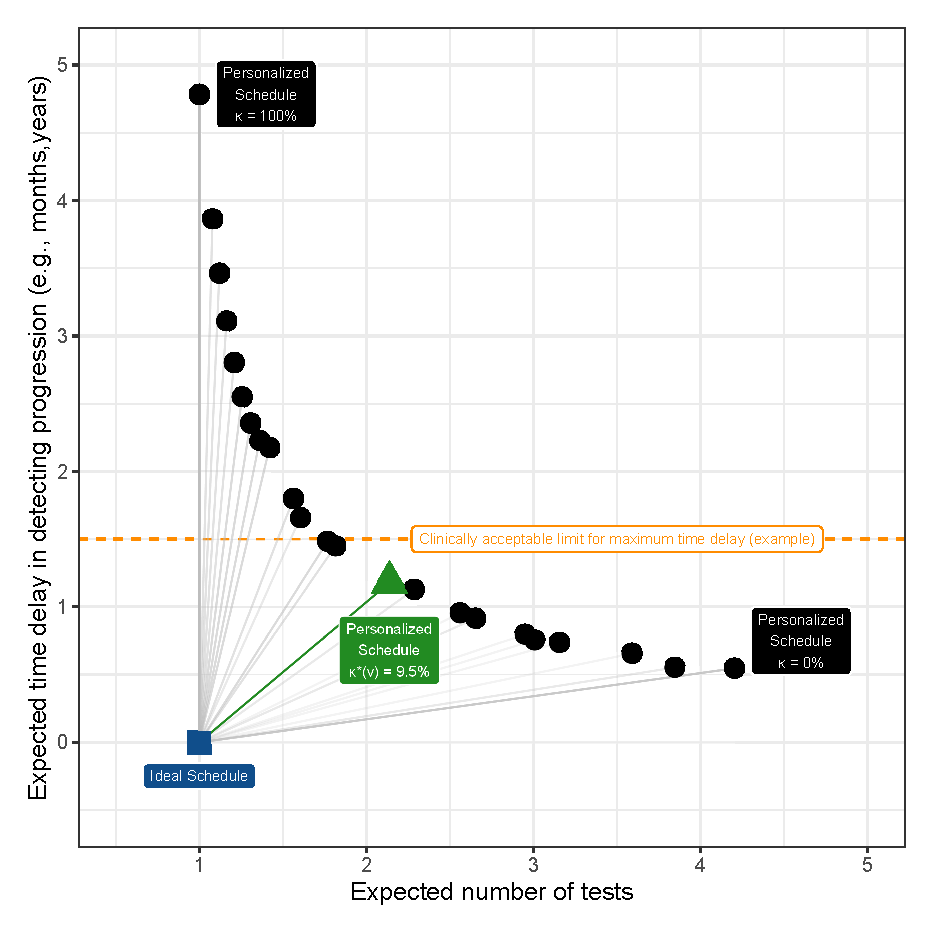
\includegraphics{images/kappa_choice_102.eps}}
\caption{\textbf{Automatic choice of risk threshold $0 \leq \kappa \leq 1$ using~(\ref{eq:kappa_choice})}. The ideal schedule of tests at point (1,0) is shown as a blue square. It plans exactly one invasive test at the true time of progression $T^*_j$ of a patient and hence leads to a zero time delay in detecting progression. Personalized schedules based on a grid of thresholds chosen between $0 \leq \kappa \leq 1$ are shown with black circles. Higher thresholds lead to fewer tests, but also higher expected time delay. We propose to choose the personalized schedule based on $\kappa_a=21.2\%$ threshold (green triangle). This is because it has the least Euclidean distance (shown with a green line) to the ideal schedule. It is also possible to find the least distance under a certain clinically acceptable limit on time delay (orange dashed line), or number of tests.}
\label{fig:kappa_choice}
\end{figure}

\subsection{Expected Time Delay in Detecting Progression}
\label{subsec:exp_delay_estimation}
Of the two measures in, we estimate the expected time delay in detecting progression $E\{Q_j(S_j^{\kappa}, t)\}$ in a patient-specific manner as well. That is, two patients may follow the same schedule, but they will expect different time delays. The calculation of the time delay is not limited to personalized schedules only, but can be done for any schedule $S$ with $N$ time points $S=\{s_1,\ldots, s_N\}$. Corresponding to each of these time points are the $N$ time intervals $s_{n-1} < T^*_j \leq s_n$ in which progression may be observed, and the $N$ possible time delays $s_n - T^*_j$, where $n=1,\ldots,N$. However, the time delay is not defined for the scenario in which the patient obtains progression after the time of the last test in the schedule $T^*_j > s_N$. The resulting definition for time delay given a schedule $S$ is:
\begin{equation}
Q_j (S, t) = \left\{ \begin{array}{lcrr}
  s_1 - T^*_j, &\mbox{if}& s_0 < T^*_j \leq s_1, &s_0=t\\
  \ldots \\
  s_N - T^*_j, &\mbox{if}& s_{N-1} < T^*_j \leq s_N  
\end{array} \right.
\end{equation}
We utilized the patient-specific expected time delay $E\{Q_j(S_j^{\kappa}, t)\}$ in~(\ref{eq:kappa_choice}). To this end, we exploit the personalized cumulative-risk profile of the patient (Equation~\ref{eq:cumulative_risk}). Specifically, the expected time delay can be calculated as the weighted sum of the $N$ conditional expected time delays, corresponding to the $N$ scenarios wherein the patient obtains progression in the intervals $s_{n-1} < T^*_j \leq s_n$, with $n=1,\ldots,N$.
\begin{equation}
\label{eq:expected_delay}
\begin{split}
E\{Q_j(S, t)\} &= \sum_{n=1}^{N} q_j(s_n, s_{n-1}) \mbox{Pr}(s_{n-1} < T^*_j \leq s_n) , \quad s_0 = t\\
q_j(s_n, s_{n-1}) &= s_n - E(T^*_j \mid s_{n-1}, s_n, v)\\
E(T^*_j \mid s_{n-1}, s_n, v) &= s_{n-1} + \int_{s_{n-1}}^{s_n} \mbox{Pr}\Big\{T^*_j \geq u \mid s_{n-1} < T^*_j \leq s_n, \mathcal{Y}_{1j}(v), \ldots, \mathcal{Y}_{Kj}(v), \mathcal{A}_n\Big\} \mathrm{d}u\\
\mbox{Pr}(s_{n-1} < T^*_j \leq s_n) &= R_j(s_n \mid t, v) - R_j(s_{n-1} \mid t, v),
\end{split}
\end{equation}
where $E(T^*_j \mid s_{n-1}, s_n, v)$ denotes the conditional expected time of progression for the scenario $s_{n-1} < T^*_j \leq s_n$, and is calculated as the area under the corresponding survival curve. The personalized expected delay has the advantage that it is updated over follow-up as more patient data becomes available. Since it can be calculated for any schedule, it can assist patients and doctors in comparing schedules before making a decision. Although, in order to have a fair comparison of expected delays between different schedules for the same patient, a compulsory test at a common horizon time point should be planned in all schedules.